\documentclass[11pt]{article}
\usepackage[margin=1in]{geometry}
\usepackage[T1]{fontenc}
\usepackage[utf8]{inputenc}
\usepackage{mathptmx}
\usepackage{microtype}
\usepackage{amsmath}
\usepackage{amssymb}
\usepackage{booktabs}
\usepackage{longtable}
\usepackage{array}
\usepackage{calc}
\usepackage{graphicx}
\usepackage{caption}
\usepackage{xcolor}
\usepackage[numbers,sort&compress]{natbib}
\usepackage[hidelinks]{hyperref}
\providecommand{\tightlist}{\setlength{\itemsep}{0pt}\setlength{\parskip}{0pt}}
\captionsetup{font=small,labelfont=bf,skip=6pt}
\setlength{\parskip}{3pt}
\title{\textbf{Evidence Availability Is Not Evidence Entitlement}\\[4pt]
\large Replayable, Evidence-Bounded Mapping of Multimodal Biomechanical Data to Clinical Assessment Criteria}
\author{Michael P.\ Ryder, DO\\ \small Independent researcher \\ \small \texttt{michaelryder.do@gmail.com}}
\date{\small Preprint --- September 2026. Pre-registered protocol; every number is read from a committed, content-addressed artifact.}
\begin{document}
\maketitle
\begin{abstract}
\noindent Clinical assessment frameworks ask for information that no single measurement modality can supply, and a computational pipeline that scores such a framework from sensor data must either impute what it cannot measure, silently narrow the framework, or state explicitly which criteria it cannot justify. We built a deterministic, content-addressed pipeline that takes the third path and evaluated it across the metadata-defined public PhysioNet One-Legged Stand Test corpus: 32 participants, 333 captures, and 1,233 of 1,238 attempts buildable from the published source files, under two acquisition protocols. The pipeline maps per-attempt event labels and force-plate centre-of-pressure measurements into criterion-level evaluations of the Morse Fall Scale and the Berg Balance Scale under versioned criterion maps; every run is identified by a composite SHA-256 over the source fixture, the canonicalization specification, the criterion map, and the harness, every evaluated criterion carries evidence pointers, and every non-evaluable criterion carries a reason. Across eight full-corpus execution contexts (986,400 executions) no output hash diverged. Determinism did not make the interpretation right; it made its errors localizable. The prespecified initial Morse mapping (v1) classified all 1,082 evaluable attempts as \emph{impaired}. Lineage separated two independent causes: the map read the wrong temporal construct (a within-attempt stable-phase window instead of the stance interval), and it gave a legitimate measurement, centre-of-pressure sway area, categorical authority that bounds drafted against synthetic fixtures could not support. Each cause was corrected by a prospectively specified map frozen before the corrected map was executed: v2 corrected the construct and added protocol censoring while deliberately retaining the sway gate, and failed as predicted (944 attempts still \emph{impaired} by sway); v2.1 removed sway's categorical authority while retaining it as linked, reported evidence, and the distribution opened without any threshold change (73 \emph{normal}, 57 \emph{weak}, 229 \emph{impaired}, 723 \emph{protocol-censored}, 151 \emph{non-evaluable}). Evaluability was bounded in three structurally distinct ways: the modality cannot observe four of six Morse items; the Morse gait item asks about ambulation, so single-leg stance is only partial evidence for it while the same measurement is derivable evidence for Berg item 14; and the dataset's 4-second cued protocol never permitted the 10-second clinical threshold to be observed, so every short-protocol attempt is censored rather than labelled; the seventeen older participants who performed both protocols were observable to the 10-second threshold under one and not the other, on the same variable. Sourcing the 4-second ceiling to the dataset's companion paper re-identified 776 fixtures and changed no label. A prespecified generality test failed: adding the Berg map required a generic ordinal rule type in the harness (86 lines), because the rule vocabulary, not the evidence machinery, had Morse's category names baked in. The contribution is a methods artifact and a replayable record of a clinical interpretation being wrong, localized, corrected without tuning, wrong again for an independent reason, corrected again, and meeting a prespecified boundary of its own generality. Nothing here claims predictive validity or clinical use.
\end{abstract}

\section{Introduction}\label{introduction}

\subsection{The problem}\label{the-problem}

A clinical assessment framework is a contract between a clinician and a body of evidence. The Morse Fall Scale [morse1989] has six items: history of falling, secondary diagnosis, ambulatory aids, intravenous therapy, gait, and mental status. Three are record fields, one requires a cognitive assessment, one is inferred from observed ambulation, and only gait bears any relationship to what a force plate or a motion-capture rig measures. Even that relationship is a proxy.

When a computational system is asked to produce a framework score from a modality that cannot supply most of the framework's inputs, it has three options: impute the missing items and emit a complete-looking score; score the derivable subset and emit it under the framework's name; or evaluate what the evidence supports, mark every other criterion non-evaluable with a stated reason, and make the coverage machine-readable. This paper builds the third option and evaluates it on a complete public corpus. The argument is not that explicit refusal is more polite. It is that a system which cannot say what it did not know cannot be replayed, audited, or recalibrated when the clinical interpretation changes, and we show, with a recorded sequence of two independent interpretive errors, that recalibration is where the property earns its keep.

\subsection{Three ways evidence falls short, and one orthogonal question}\label{three-ways-evidence-falls-short-and-one-orthogonal-question}

The executed study produced a taxonomy that the pre-registration did not anticipate in full. Evaluability of a clinical criterion from a measurement modality is bounded by three structurally distinct conditions:

\begin{enumerate}
\def\labelenumi{\arabic{enumi}.}
\tightlist
\item
  \textbf{Modality compatibility.} Can the sensor observe the required evidence at all? Four Morse items and nine Berg items are non-evaluable from single-leg-stance biomechanics for this reason.
\item
  \textbf{Framework (construct) compatibility.} Is the measured quantity the construct the criterion asks about? The Morse gait item describes ambulation; single-leg stance is related evidence, not that observation. Berg item 14 \emph{is} single-leg stance. The same measurement is partial evidence for one and derivable evidence for the other.
\item
  \textbf{Protocol compatibility.} Did the acquisition procedure permit the criterion's boundary to be observed? A 4-second cued stance cannot establish whether a participant could stand for 10 seconds. That is censoring, not failure, and the label is withheld.
\end{enumerate}

Orthogonal to all three is \textbf{evidentiary authority}: a quantity can be legitimate, measured, provenance-linked evidence without being entitled to determine a clinical category. Centre-of-pressure sway area is a valid measurement; 600 mm$^{2}$ is not thereby a Morse gait boundary. Section 4.4 shows the difference operationally.

\subsection{What the pipeline produces}\label{what-the-pipeline-produces}

Over the PhysioNet OLST dataset [copeland2026scidata], for each attempt the pipeline produces a canonical JSON fixture whose bytes are stable across executions (invariant O-CI-0); up to four Evidence Modality Units (EMUs) carrying \texttt{non\_authoritative=true}, \texttt{requires\_human\_ack=true}, attempt-level provenance, and a payload hash, with any EMU whose required source is absent omitted rather than imputed; a criterion-by-criterion evaluation under a versioned criterion map, with labels and evidence pointers for evaluated criteria, a \texttt{protocol\_censored} state where the acquisition ceiling withholds a label, and a \texttt{non\_evaluable\_reason} for the rest; and a composite \texttt{run\_id} over the execution context together with an \texttt{output\_hash} over the result.

\subsection{Contributions}\label{contributions}

\begin{enumerate}
\def\labelenumi{\arabic{enumi}.}
\tightlist
\item
  \textbf{An evidence-bounded mapping architecture} in which criterion coverage is a declared, machine-readable output, non-evaluable criteria carry reasons, and protocol censoring is a distinct state from both a label and a gap (Sections 3.4--3.7).
\item
  \textbf{Content-addressed replay with source lineage} from the dataset's per-file digests through the canonicalization specification, criterion map, and harness source to the output, verified rather than assumed: 986,400 real-data executions across eight contexts with zero divergence, and a store from which every stored run replays bit-for-bit (Sections 3.8--3.9, 4.1).
\item
  \textbf{Protocol censoring of a measured construct relative to a clinical threshold}, with the acquisition ceiling carried in the fixture as a sourced fact (Sections 3.2, 4.3). Seventeen participants are observable to 10 s under one protocol and not the other, on the same variable.
\item
  \textbf{A recorded, prospectively specified recalibration sequence}: v1 $\rightarrow$ v2 $\rightarrow$ v2.1, each correction triggered by evidence available before the corrected map was frozen, with the historical results preserved and the cause of each divergence attributable from digests alone (Sections 3.6, 4.4, 4.5).
\item
  \textbf{A prespecified generality test that failed and was reported as promised.} The frozen protocol required that a second framework be added with zero harness change. It could not be: Berg item 14 needed a generic ordinal rule type (86 lines added, 7 removed). The evidence representation, loader, canonicalization, store, and fixture set were untouched; the rule vocabulary was framework-specific (Section 4.6). The original claim is withdrawn.
\end{enumerate}

\subsection{What this paper does not claim}\label{what-this-paper-does-not-claim}

The pipeline does not predict falls. No label is clinically validated. Every category emitted under any map is a proxy category under that map's declared rule, not a Morse gait classification or a Berg score in the instrument's own sense, and a cleaner mapping is still a proxy. Deterministic output is not clinically correct output; determinism is what makes correctness checkable. Section 6 states these boundaries in full.

\section{Related Work}\label{related-work}

\emph{(Wording follows the structured literature checkpoint of 2026-09-09, \texttt{paper/literature\_review/}; bracketed keys resolve in its \texttt{.bib}. Two claims from the frozen draft are deleted on its recommendation: the ``no prior system combines\ldots{}'' gap sentence and the ``first public corpus'' sentence, which is the dataset authors' claim to make.)}

\textbf{Automating clinical scales from sensors.} Berg Balance Scale scores or BBS-defined risk categories have been estimated from accelerometers, wearable IMUs, depth cameras and an instrumented Timed Up and Go [badura2016bbs; kim2021bbs; eichler2022bbs; lu2025bbs; zhang2026bbs], and single-leg stance has been timed from video and used alone as a proxy for fall-risk category [kawa2018sls; tripathy2018sls]. These systems ask how much of a clinician's score can be predicted from limited observations; items that cannot be observed are dropped, regressed through a proxy, or noted as a limitation, not represented as an output. Item-level crosswalks between mobility instruments succeed for a minority of items [stenum2025mfs], and for the Morse Fall Scale the item no sensor observes, fall history, is the one that discriminates fallers [oppegaard2026mfs]. We ask the inverse question, which criteria the observations are entitled to support, and make the answer machine-readable.

\textbf{Abstention and determinability.} The reject option and selective prediction let a model decline to answer when its confidence or expected cost warrants [chow1970; elyaniv2010; geifman2017; mozannar2020], and have been applied to clinical extraction and risk models [kompa2021; swaminathan2023]. ClinDet-Bench shows that determinability of a clinical score under missing items is a logical property of the evidence rather than of model confidence [watanabe2026clindet]; a deployed radiology decision-support system that emitted ``indeterminate (insufficient information)'' separately from ``not validated'' showed that the handling of such states dominates downstream behaviour [schneider2015]. Our \texttt{non\_evaluable} and \texttt{protocol\_censored} states are neither uncertainty nor cost: the criterion is inadmissible because the modality, the construct, or the acquisition protocol cannot supply the required evidence, and no calibration changes that.

\textbf{Missingness.} The dominant treatments of missing clinical data are imputation and the modelling of informative missingness [rubin1976; che2018grud; agniel2018; groenwold2020; mitra2023]. The distinction between \emph{not applicable} and \emph{unknown} exists at the datum level in HL7 NullFlavor and FHIR data-absent-reason [hl7nullflavor; fhirdataabsent], at instrument level in scale-specific invalidation rules [goetz2015mdsupdrs], and in causal inference as structural versus random positivity violations [westreich2010positivity]. We carry that distinction to the level of an instrument criterion evaluated from a measurement modality, and separate three structural causes.

\textbf{Declared evidentiary entitlement.} Computable-eligibility research classifies which trial criteria can be resolved from EHR data at design time [weng2010; ross2010; kopcke2013; raghavan2015; muqeeth2026]; Bouzinier et al.~assert, per decision rule, which evidence types the rule may use and validate rules prospectively against that specification [bouzinier2026]; Quant ES computes per-variant evidence availability against hashed rule sets before interpretation [saadat2025quantes]. Concurrently, EviBound fixes a protocol-conditioned claim-permission matrix before inference for speech-based screening [gao2026evibound]. We share the declare-before-inference stance and differ in the unit and the object: derivability is declared per clinical criterion, evaluated per case against the evidence actually present, an acquisition ceiling is treated as censoring of a measured construct relative to a numeric threshold, and the declaration is bound to the result's identity. Inferential validity, whether a measure supports a conclusion, has been proposed as a validity concept for digital measures [tekwe2026]; the criterion map is an executable instance of it.

\textbf{Provenance and versioned interpretation.} Provenance capture for clinical data and decision support is mature [w3cprov; curcin2017jbi; gierend2024], and AI decision-support guidance requires it [labkoff2024; lekadir2025futureai]. That definitions change results is documented: successive quality-measure versions re-executed on the same data shift measured prevalence [cholan2017amia; cholan2017egems], phenotype edits move incidence rates [makadia2023], and independent implementations of one cohort description diverge [ostropolets2023]. Hash-identified rule sets, clinical assertions and data exist separately [saadat2025quantes; cao2026tracegraph; wack2025gitommix]. What we add is the identity decomposition: source evidence, canonicalization, criterion map and harness each carry a content-addressed identity, the historical result remains reproducible by construction when the map changes, and the cause of any divergence is attributable by comparing digests without re-deriving either result.

\textbf{Balance assessment and the OLST.} Single-leg stance norms and cut-offs are protocol- and population-dependent [springer2007; bohannon2006; vereeck2008; araujo2022; beauchamp2022; chung2025], ceiling effects are a recognised measurement property [terwee2007; mokkink2010cosmin], and a 10 s ceiling has been noted to hide subtle imbalance [deabreu2024]. The PhysioNet OLST dataset [copeland2026scidata; copeland2026gaitposture] provides synchronized motion capture, force plates and radar with per-attempt event labels under two acquisition protocols; we use it as a substrate for testing evidence-bounded mapping and replay, and defer outcome claims.

\section{Methods}\label{methods}

\subsection{Dataset and corpus inventory}\label{dataset-and-corpus-inventory}

The PhysioNet OLST dataset (release 1.0, DOI 10.13026/46hn-6b25) contains 32 healthy participants, 15 young ($\leq$32 y) and 17 older ($\geq$64 y), performing the One-Legged Stand Test. \texttt{Metadata/OLST\_Attempts.csv} is the system of record for attempt timing, with four events per attempt in MoCap-clock seconds: foot-lift (\texttt{t\_foot\_up}), start of stability (\texttt{t\_stable}), end of stability (\texttt{t\_break}), and foot-touchdown (\texttt{t\_end}). Each capture provides a motion-capture CSV (100 Hz) and two force-plate CSVs (1200 Hz, one per plate). The published \texttt{SHA256SUMS.txt} is the root of source lineage. Radar range-Doppler maps are not used.

Two acquisition protocols are encoded in the capture identifier's movement code. \texttt{MNTRL}/\texttt{MNTRR} (``Mountain-to-Tree'', left/right base) are cued short trials; \texttt{TRLGL}/\texttt{TRLGR} are 20-second sustained-balance trials performed by the older cohort only. The README states the 20-second protocol; the companion paper states both: ``short (4 s) and long (20 s) OLST trials'' [copeland2026gaitposture]. Base leg for the \texttt{TRLG*} codes was verified from force-plate vertical load rather than assumed from the letter.

\begin{longtable}[]{@{}
  >{\raggedright\arraybackslash}p{(\linewidth - 2\tabcolsep) * \real{0.5000}}
  >{\raggedright\arraybackslash}p{(\linewidth - 2\tabcolsep) * \real{0.5000}}@{}}
\toprule\noalign{}
\begin{minipage}[b]{\linewidth}\raggedright
Item
\end{minipage} & \begin{minipage}[b]{\linewidth}\raggedright
Count
\end{minipage} \\
\midrule\noalign{}
\endhead
\bottomrule\noalign{}
\endlastfoot
Participants (young / older) & 32 (15 / 17) \\
Captures after the published exclusion \texttt{12\_MNTRL\_V2} & 333 \\
Captures by protocol: MNTR young / MNTR older / TRLG older & 88 / 121 / 124 \\
Attempt rows & 1,238 \\
Attempts built & 1,233 \\
Attempts not buildable (\texttt{35\_MNTRL\_V4}: force-plate files absent from the release manifest) & 5 \\
Attempts per capture & 1 to 15 (median 3) \\
Attempts with no \texttt{t\_stable} event (never reached stability) & 151, all older \\
Attempts with an attempt window overlapping another in its capture & 2 captures (\texttt{47\_TRLGL\_V4}, \texttt{56\_TRLGL\_V4}) \\
\end{longtable}

Every referenced source file was verified against the manifest before any fixture was built: 997 of 999 files present and matching, the two absent files being the manifest gap above.

\subsection{Canonicalization and the acquisition ceiling}\label{canonicalization-and-the-acquisition-ceiling}

The canonicalization specification fixes lexicographic key order, six-decimal float representation with \texttt{NaN}/\texttt{Inf} rejected in favour of \texttt{null} plus a \texttt{\textless{}field\textgreater{}\_\_missing\_reason}, and event windows in milliseconds. Two windows are derived per attempt: the \textbf{stable phase} \texttt{t\_stable\ $\rightarrow$\ t\_break} (or \texttt{t\_end} when \texttt{t\_break} is empty), over which centre-of-pressure quantities are computed, and, from specification v1.3, the \textbf{stance interval} \texttt{t\_foot\_up\ $\rightarrow$\ t\_end}. An attempt with no \texttt{t\_stable} is still canonicalized: its stable phase and force-plate block are \texttt{null} with reasons, its stance interval is present.

The fixture also carries an \texttt{acquisition\_protocol} block: the movement code, an \texttt{observation\_ceiling\_ms}, and the source of that ceiling. The ceiling is an acquisition fact, never inferred from the data. Under specification v1.3 it was \texttt{20000} for \texttt{TRLG*} (README) and \texttt{null} for \texttt{MNTR*} (the README does not state the cue). Under specification v1.4 it is \texttt{4000} for \texttt{MNTR*}, sourced to the companion paper. The fixture builder uses correctly rounded summation so that fixture bytes do not depend on the interpreter (Python 3.12 changed built-in \texttt{sum()}; the pilot fixtures, built on 3.9, differed in the last bits of three floats from a 3.14 rebuild; output hashes were never affected because canonicalization rounds to six decimals, but fixture identities were).

\subsection{Evidence Modality Units}\label{evidence-modality-units}

\begin{longtable}[]{@{}
  >{\raggedright\arraybackslash}p{(\linewidth - 4\tabcolsep) * \real{0.3333}}
  >{\raggedright\arraybackslash}p{(\linewidth - 4\tabcolsep) * \real{0.3333}}
  >{\raggedright\arraybackslash}p{(\linewidth - 4\tabcolsep) * \real{0.3333}}@{}}
\toprule\noalign{}
\begin{minipage}[b]{\linewidth}\raggedright
EMU
\end{minipage} & \begin{minipage}[b]{\linewidth}\raggedright
Payload
\end{minipage} & \begin{minipage}[b]{\linewidth}\raggedright
Required source
\end{minipage} \\
\midrule\noalign{}
\endhead
\bottomrule\noalign{}
\endlastfoot
\texttt{gait\_temporal\_control} & \texttt{stability\_duration\_ms} (stable phase, when present), \texttt{stance\_duration\_ms} (stance interval), \texttt{observation\_ceiling\_ms}, \texttt{protocol\_code}, \texttt{trial\_leg} & event labels \\
\texttt{postural\_stability\_index} & \texttt{mean\_cop\_displacement\_mm}, \texttt{sway\_area\_mm2} (95 \% confidence ellipse), a legacy field & force-plate CoP over the stable phase \\
\texttt{weight\_distribution\_asymmetry} & \texttt{left\_pct}, \texttt{right\_pct}, \texttt{asymmetry\_index} & bilateral \texttt{Force\_Z} over the stable phase \\
\texttt{balance\_control\_quality} & \texttt{composite\_score} & derived; requires the first two \\
\end{longtable}

An EMU whose required source is absent is omitted. For the 151 attempts with no stable phase, \texttt{gait\_temporal\_control} is emitted with the stance interval only and no CoP EMU exists. Fields added at v1.3 appear only when the fixture carries their source, which is what kept every pre-existing golden hash valid.

\subsection{Criterion maps}\label{criterion-maps}

A criterion map is a versioned JSON document that declares, for each item of a target framework, the required EMUs, a derivability class (\texttt{derivable}, \texttt{partial}, \texttt{non\_evaluable}), an optional rule block, and reasons. Its SHA-256 (\texttt{criterion\_map\_id}) enters the \texttt{run\_id}, so a map revision is a new execution context by construction. A map may also declare a capture-level \texttt{aggregation} rule; aggregation is never a silent merge. Maps are never edited after execution; a change is a new file.

\subsection{Morse Fall Scale maps: the executed chronology}\label{morse-fall-scale-maps-the-executed-chronology}

Four of six Morse criteria are non-evaluable from biomechanics under every map (history of falling, secondary diagnosis, IV therapy, mental status: record, self-report, or cognitive assessment required); ambulatory aids is \texttt{partial}. The maps differ only in the gait item.

\begin{longtable}[]{@{}
  >{\raggedright\arraybackslash}p{(\linewidth - 12\tabcolsep) * \real{0.1429}}
  >{\raggedright\arraybackslash}p{(\linewidth - 12\tabcolsep) * \real{0.1429}}
  >{\raggedright\arraybackslash}p{(\linewidth - 12\tabcolsep) * \real{0.1429}}
  >{\raggedright\arraybackslash}p{(\linewidth - 12\tabcolsep) * \real{0.1429}}
  >{\raggedright\arraybackslash}p{(\linewidth - 12\tabcolsep) * \real{0.1429}}
  >{\raggedright\arraybackslash}p{(\linewidth - 12\tabcolsep) * \real{0.1429}}
  >{\raggedright\arraybackslash}p{(\linewidth - 12\tabcolsep) * \real{0.1429}}@{}}
\toprule\noalign{}
\begin{minipage}[b]{\linewidth}\raggedright
Map
\end{minipage} & \begin{minipage}[b]{\linewidth}\raggedright
Specified
\end{minipage} & \begin{minipage}[b]{\linewidth}\raggedright
Gait derivability
\end{minipage} & \begin{minipage}[b]{\linewidth}\raggedright
Duration construct
\end{minipage} & \begin{minipage}[b]{\linewidth}\raggedright
Sway
\end{minipage} & \begin{minipage}[b]{\linewidth}\raggedright
Censoring
\end{minipage} & \begin{minipage}[b]{\linewidth}\raggedright
Aggregation
\end{minipage} \\
\midrule\noalign{}
\endhead
\bottomrule\noalign{}
\endlastfoot
v1 & before any real data (May 2026) & derivable & stable phase \texttt{t\_stable\ $\rightarrow$\ t\_break} & gates: \texttt{normal} needs \textless{} 250 mm$^{2}$, $\geq$ 600 mm$^{2}$ forces \texttt{impaired} & none & none \\
v2 & 2026-09-09, after D1, before any real v2 run & partial & stance \texttt{t\_foot\_up\ $\rightarrow$\ t\_end} & gates retained unchanged & yes & best-of-attempts, overlap check \\
v2.1 & 2026-09-09, after the v1 full-corpus run, before any real v2 or v2.1 run & partial & stance & reported, required as linked evidence, not gating & yes & as v2 \\
\end{longtable}

Duration thresholds are 10 s / 5 s in every map and were never changed. The v2 map deliberately kept the v1 sway gate: it was frozen before the full-corpus v1 result existed, and the protocol's Step 0.5 rule was that a frozen map is executed as frozen and any later change is a new dated map.

\textbf{Protocol censoring rule (D4a).} When the acquisition ceiling is below a threshold the label would need, the attempt is \texttt{protocol\_censored}; the measured duration is reported in the evaluation detail, and no duration label is asserted. A null ceiling censors every attempt. Under v2 the sway gate could still force \texttt{impaired} on a censored attempt; under v2.1 nothing overrides censoring. The prespecified reading of the 4-second cue (A14, stated before execution) is that no duration threshold is observable under it, so the sourced ceiling and the null ceiling yield the same decision.

\textbf{Aggregation (D2).} OLST is conventionally recorded as the best of several attempts. v2 and v2.1 declare \texttt{best\_of\_attempts\ =\ max(stance\_duration\_ms)} per capture, evaluable only if every attempt yields the field, and non-evaluable when any two attempt windows overlap (D2a). Sway never enters the aggregate.

\subsection{Berg Balance Scale map}\label{berg-balance-scale-map}

Item text was verified against the Academy of Neurologic Physical Therapy \emph{Core Measure: Berg Balance Scale} document, reprinted from the author (J Neurol Phys Ther 2018;42:174-220). Item 14, \emph{standing on one leg}: 4 ``able to lift leg independently and hold \textgreater{} 10 seconds''; 3 ``5--10 seconds''; 2 ``$\geq$ 3 seconds''; 1 ``tries to lift leg unable to hold 3 seconds but remains standing independently''; 0 ``unable to try or needs assist to prevent fall''. The map declares 9 items non-evaluable (transfers, reaching, turning, stepping: not elicited), 4 partial (items 2, 6, 7, 13: a different stance condition, named in the reason), and item 14 derivable from \texttt{gait\_temporal\_control} alone, because the rubric is a duration rubric and sway is not part of it. Levels are \texttt{score\_4} $\geq$ 10,001 ms (strictly \textgreater{} 10 s in integer milliseconds), \texttt{score\_3} $\geq$ 5,000, \texttt{score\_2} $\geq$ 3,000, and a floor label \texttt{score\_1\_or\_0\_unresolved}: every attempt has a foot-lift, so ``unable to try'' does not apply, but the release annotates no assistance or loss of balance, so 1 and 0 cannot be separated and the map refuses to choose. Censoring applies: a level is emitted only when every boundary needed to place the duration in it was observable under the ceiling.

\subsection{Replay harness, identity scheme, and store}\label{replay-harness-identity-scheme-and-store}

\texttt{run(fixture\_path,\ mapping\_spec\_version)} computes \texttt{fixture\_id\ =\ SHA-256(bytes)}, applies the exclusion gates, canonicalizes, derives EMUs, resolves the map file from the version (an unknown version raises; there is no fallback), evaluates, and computes \texttt{output\_hash} over the canonical result including traceability, and \texttt{run\_id} over \texttt{\{fixture\_id,\ dataset\_version,\ mapping\_spec\_version,\ spec\_id,\ criterion\_map\_id,\ harness\_version\}}. \texttt{spec\_id} and \texttt{criterion\_map\_id} are read from disk on every call; \texttt{harness\_version} is digested at import. Real-data fixtures pin the manifest digests of every source file read.

The store is six JSONL streams keyed by content hash (runs, EMUs, evaluations, non-evaluables, fixture text, capture aggregates). Ingest is idempotent; \texttt{recall} rebuilds a report without execution; \texttt{verify\_replay} re-executes the stored fixture text and asserts output-hash equality.

\subsection{Comparator and metrics}\label{comparator-and-metrics}

The naive comparator applies the 10 s / 5 s cutoffs to the stable-phase window, defaults absent values to zero, and emits a label with no evidence pointers; it is the shape of a reasonable first implementation. Metrics: distinct \texttt{output\_hash} values per fixture over N executions (target 1); evidence-pointer coverage on evaluated lines and reason coverage on non-evaluable lines (target 100 \%); comparator agreement; and, across map versions over the same fixture, equal \texttt{fixture\_id}, \texttt{spec\_id}, and \texttt{harness\_version} with distinct \texttt{criterion\_map\_id} and \texttt{run\_id}.

\subsection{Pre-registration and amendment discipline}\label{pre-registration-and-amendment-discipline}

The manuscript draft and analysis plan were committed (\texttt{af1fc973}) before the D1 distributions were computed. Every later decision is a dated entry in one amendment file with the commit that executed it. The chronology that matters for the interpretation claims is: D1 computed after the freeze (\texttt{e293265f}); harness frozen and v2 specified before any real v2 run (\texttt{7252ce6c}, \texttt{950e04b4}); Step 1 v1 executed (\texttt{044335b2}); v2.1 specified from the v1 full-corpus evidence, before any real v2 or v2.1 run (\texttt{a722c193}); v2 and v2.1 executed as frozen (\texttt{6a60385a}); the 4-second ceiling sourced and re-executed (\texttt{aab36f0f}, \texttt{049fd548}); Berg specified and executed (\texttt{8727fd5e}, \texttt{23c42011}). No map was designed from the output of the map it replaced.

\section{Results}

\begin{figure}[t]
\centering
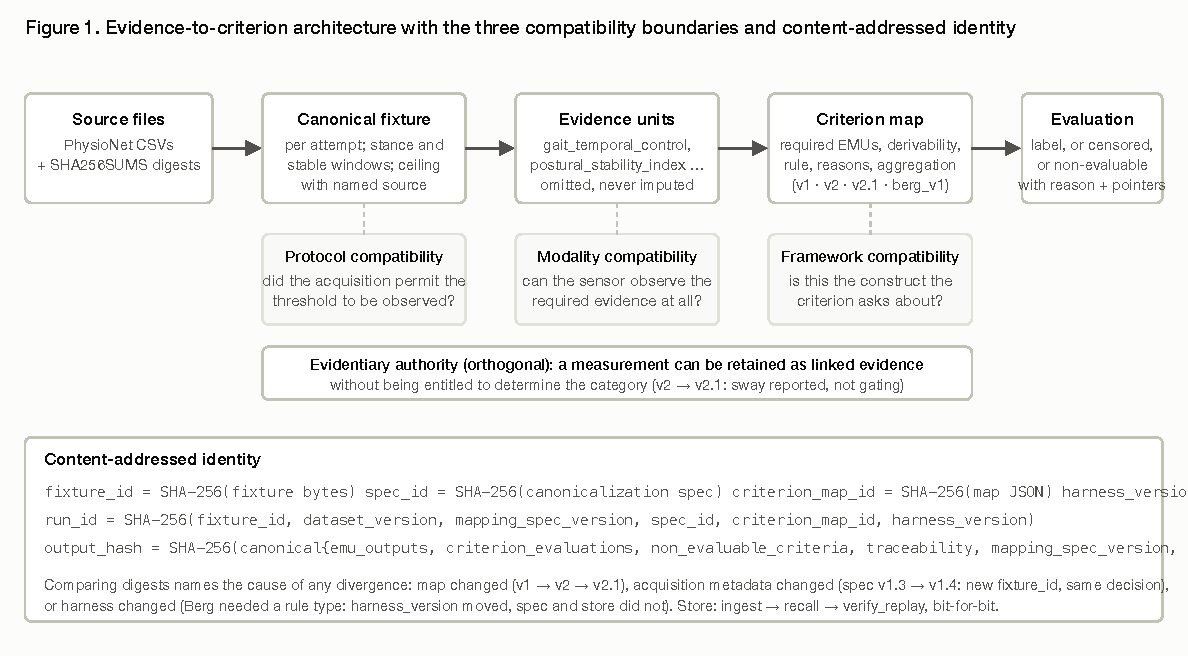
\includegraphics[width=\textwidth]{figs/fig1_architecture.pdf}
\caption{Evidence-to-criterion architecture. Source files with manifest digests are canonicalized per attempt (both windows, sourced ceiling) into Evidence Modality Units (omitted, never imputed) and evaluated under a versioned criterion map, with three compatibility boundaries and an orthogonal authority question.}
\label{fig:architecture}
\end{figure}

\begin{figure}[t]
\centering
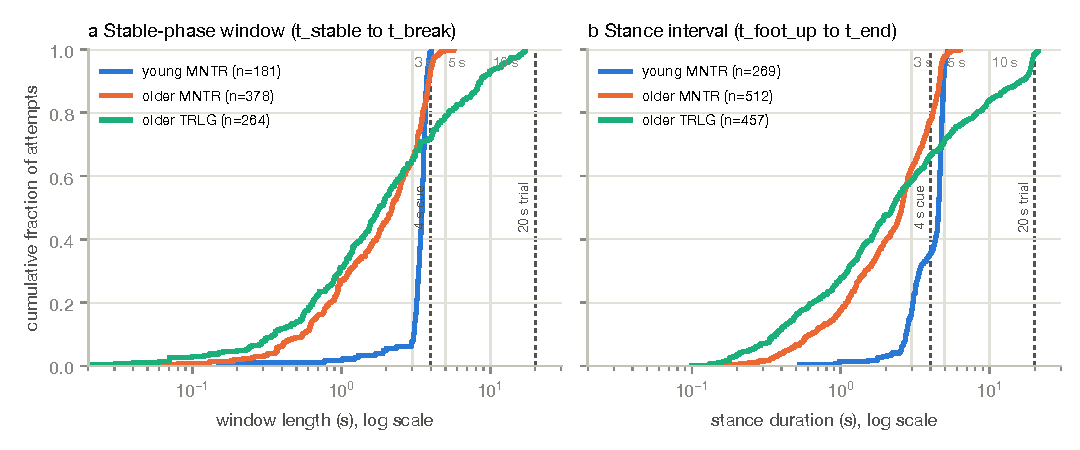
\includegraphics[width=\textwidth]{figs/fig2_duration_constructs.pdf}
\caption{Duration constructs by acquisition protocol. Empirical cumulative distributions per attempt of (a)~the stable-phase window and (b)~the stance interval, log scale, with the 3, 5, and 10\,s boundaries and the 4\,s cue and 20\,s trial marked.}
\label{fig:duration}
\end{figure}

\begin{figure}[p]
\centering
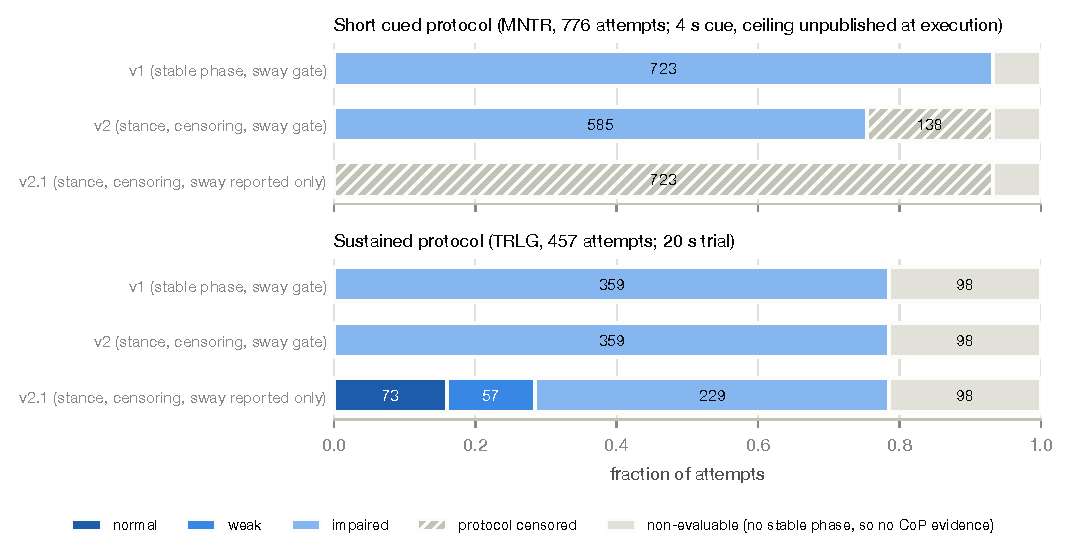
\includegraphics[width=\textwidth]{figs/fig3_versioned_recalibration.pdf}
\caption{The versioned recalibration. Per-attempt label composition under v1, v2, and v2.1 for the cued and sustained protocols.}
\label{fig:recal}
\end{figure}

\begin{figure}[t]
\centering
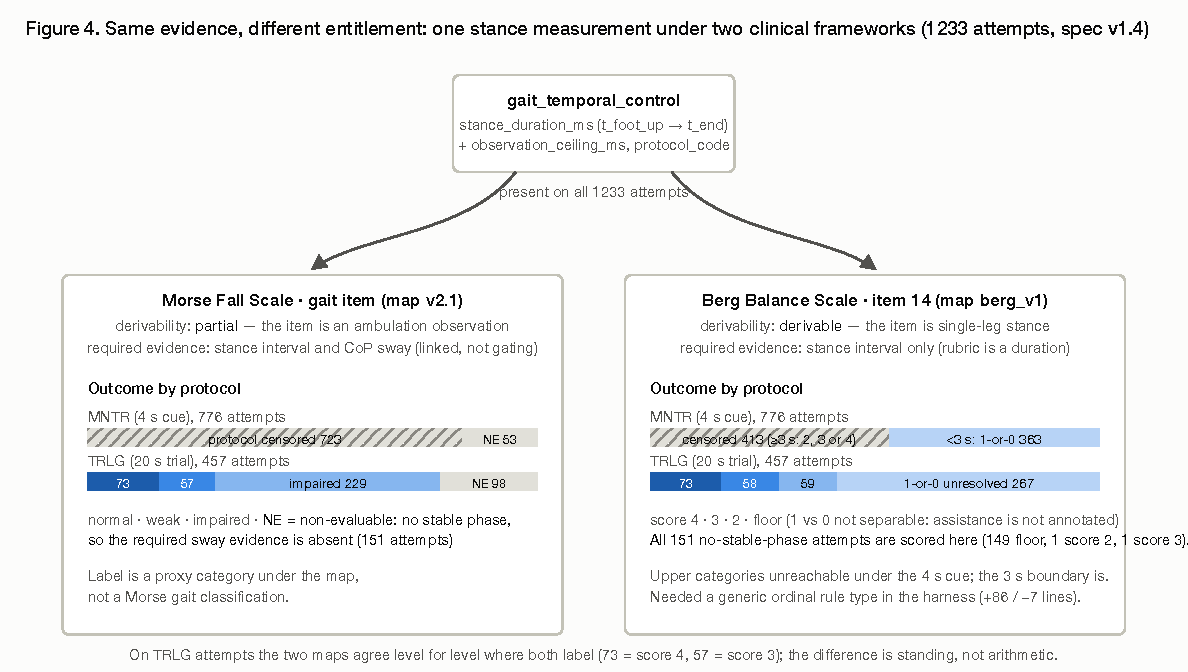
\includegraphics[width=\textwidth]{figs/fig4_same_evidence_different_entitlement.pdf}
\caption{Same evidence, different entitlement. One stance duration feeding the Morse gait item (partial; sway required as linked evidence) and Berg item 14 (derivable; stance only).}
\label{fig:entitlement}
\end{figure}
\label{results}

Figures: Figure 1 (architecture and the three boundaries), Figure 2 (duration constructs by protocol), Figure 3 (the versioned recalibration), Figure 4 (same evidence under two frameworks). All numbers are reproducible from the tagged artifact; the store tests run from a clean clone without the PhysioNet data.

\subsection{Replay and deterministic execution}\label{replay-and-deterministic-execution}

Each full-corpus context executed 1,233 fixtures 100 times: eight contexts (v1 at two harness versions and two specification versions, v2 and v2.1 at two specification versions, Berg), 986,400 executions, zero fixtures with more than one output hash, in addition to the pilot's 19,000 synthetic and 2,000 real executions. The committed store holds 9,892 runs, 1,328 capture aggregates, and 2,037 distinct fixture texts (62 MB); a seeded sample of stored runs replays bit-for-bit in the test suite and the full store replays under an environment flag. A one-line harness change made for v2.1 (a rule flag) was shown inert for v1 empirically: the v1 corpus rerun under the new harness reproduced all 1,233 Step 1 output hashes with different \texttt{run\_id}s. Every context's \texttt{harness\_version} and \texttt{spec\_id} were verified against the on-disk digests before and after execution, and no mixed-harness run was admitted to the store.

Evidence-pointer coverage on evaluated criterion lines and reason coverage on non-evaluable lines were 100 \% in every context; the governed pipeline emitted 3,397 evidence pointers per Morse context, the comparator zero.

\subsection{Temporal construct mismatch}\label{temporal-construct-mismatch}

The prespecified initial map read the stable-phase window as the stance duration. D1 computed both windows over the corpus (Figure 2). Per attempt, the stable-phase window has a median of 3.48 s in the young cohort with no attempt at or above 5 s, and the stance interval a median of 4.53 s with a maximum of 5.28 s; in the older cohort the stance interval spreads to 21.31 s with 73 attempts at or above 10 s. \texttt{t\_break} is empty on 415 attempts, including every young final attempt, so the stable-phase window cannot support the best-of aggregate on any young capture, whereas the stance interval is present on all 1,238. The stance interval \texttt{t\_foot\_up\ $\rightarrow$\ t\_end} is the one-legged stance by the dataset's own event definitions, and where the protocol permitted sustained stance it behaves like one. D1 was resolved as a construct correction, and the stable phase was retained for the CoP quantities, where stable-phase semantics are the right ones.

\subsection{The acquisition protocol bounds clinical evaluability}\label{the-acquisition-protocol-bounds-clinical-evaluability}

The plan's decision rule expected the young cohort mostly above 10 s. It never exceeds 5.3 s, and the cause is the protocol, not the cohort. Older participants performed both protocols: their MNTR attempts have the same ceiling (maximum 6.34 s over 512 attempts, none at 10 s), and their TRLG attempts reach 21.31 s. Best-of-capture stance duration under the sustained protocol reaches 10 s in 72 of 124 captures; under the cued protocol in 0 of 209. Seventeen participants are therefore observable to the clinical threshold under one capture type and not the other, on the same variable, in the same session series.

The 4-second cue is not stated in the dataset README. It was carried as \texttt{null} at execution (specification v1.3) and sourced afterwards to the companion paper (v1.4). Observed maxima exceed the nominal cue under both protocols (6.34 s against 4 s; 21.31 s against 20 s): the ceiling is the instructed duration, the longest the protocol asked for, and the censoring rule treats it as such.

Under every censoring-aware map, all 208 cued-protocol captures with built attempts are \texttt{protocol\_censored} at the capture level, and every one of the 723 evaluable cued-protocol attempts is censored under v2.1. The 10-second distinction is exercised only on the sustained protocol.

\subsection{Reproducibility exposes interpretive error; it does not prevent it}\label{reproducibility-exposes-interpretive-error-it-does-not-prevent-it}

\textbf{v1 on the full corpus.} All 1,082 evaluable attempts were \texttt{impaired} (151 non-evaluable: no stable phase, so no CoP evidence). The comparator, reading the same stable-phase window with duration only, produced 66 \texttt{normal} and 54 \texttt{weak}, so the collapse was not caused by the duration construct alone. Every one of the 120 disagreements was forced by the sway gate: no attempt with a stable phase of 10 s or more had a sway area below 825 mm$^{2}$ (median 1,789 mm$^{2}$), and over all 1,082 attempts only 104 fell below the 250 mm$^{2}$ \texttt{normal} bound, 97 of them stable windows shorter than one second, while 864 exceeded 600 mm$^{2}$. The bounds had been drafted against synthetic fixtures with sway areas of 140--250 mm$^{2}$ for clean cases and 480--540 mm$^{2}$ for ``noisy'' cases. The synthetic suite had been built to establish software behaviour; it was never a calibration dataset. A synthetic test suite can establish software behaviour without establishing clinical calibration.

\textbf{v2 as frozen.} v2 corrected the construct and added censoring but kept the sway gate. It behaved exactly as its specification implied: the sway gate forced \texttt{impaired} on 944 attempts, all 359 evaluable TRLG attempts and 585 of 723 MNTR attempts, and only the 138 MNTR attempts with sway below 600 mm$^{2}$ reached \texttt{protocol\_censored}. A prospectively specified correction of one semantic error did not rescue an independently miscalibrated component. That is reported as the preregistered result, not as a failed experiment.

\textbf{v2.1.} With sway retained as required, pointer-linked, reported evidence but removed from label determination, and no threshold changed, the distribution opened: \texttt{normal} 73, \texttt{weak} 57, \texttt{impaired} 229 on the sustained protocol; \texttt{protocol\_censored} 723 on the cued protocol; \texttt{non\_evaluable} 151 as before (Figure 3). Recalibration did not discard evidence; it changed what the evidence was permitted to decide. Comparator agreement fell from 962 of 1,233 (v1) to 824 (v2) to 340 (v2.1), because the comparator thresholds the stable-phase window with no censoring and no evidence requirement, so agreement falls as the governed mapping stops sharing its errors.

\textbf{Capture aggregates} (identical under v2 and v2.1, since sway never entered them): cued protocol 208 captures censored; sustained protocol \texttt{normal} 71, \texttt{weak} 33, \texttt{impaired} 18; two captures withheld because attempt windows overlap. One of the two (\texttt{56\_TRLGL\_V4}, a 350 ms boundary overlap) was not found by the manual attempt-order check performed at D1 time; the frozen pairwise overlap rule found it. No tolerance was added.

\subsection{Better acquisition metadata changes evidence identity, not the decision}\label{better-acquisition-metadata-changes-evidence-identity-not-the-decision}

Sourcing the cued-protocol ceiling (v1.3 \texttt{null} $\rightarrow$ v1.4 \texttt{4000\ ms}, with the companion-paper citation carried in the fixture) and re-executing v1, v2, and v2.1 under the same harness and maps: the 776 MNTR fixtures received new \texttt{fixture\_id}s, the 457 TRLG fixtures were byte-identical with identical output hashes, every \texttt{run\_id} changed through the specification digest, and the label was unchanged on 1,233 of 1,233 attempts under each of the three maps. Same measurements, better acquisition metadata, new evidence identity, same decision; the identity decomposition names the cause of every difference.

\subsection{The same evidence has different standing under different frameworks}\label{the-same-evidence-has-different-standing-under-different-frameworks}

Berg item 14 was executed on the v1.4 fixtures (Figure 4). Every built attempt was scored or censored: \texttt{score\_4} 73, \texttt{score\_3} 58, \texttt{score\_2} 59, floor 630, \texttt{protocol\_censored} 413. Under the 4-second cue the 3-second boundary is observable while the 5- and 10-second boundaries are not, so cued-protocol attempts shorter than 3 s are placed at the floor (363) and those reaching 3 s are censored (413): no upper Berg category is reachable under the short protocol. On the sustained protocol the two frameworks agree level for level where both label (73 \texttt{normal} = \texttt{score\_4}; 57 \texttt{weak} = \texttt{score\_3}), because both read \texttt{stance\_duration\_ms} and the boundaries coincide except that Berg adds 3 s and requires strictly more than 10 s. The difference is standing, not arithmetic: Morse gait is \texttt{partial} and its map requires the sway EMU as linked evidence, so the 151 attempts with no stable phase are non-evaluable for it under every Morse map; Berg item 14 is \texttt{derivable} from the stance interval alone, and all 151 are scored (149 floor, 1 \texttt{score\_2}, 1 \texttt{score\_3}). The measurement did not change between frameworks; what it is entitled to establish did.

\textbf{The prespecified generality test failed.} The frozen protocol required the second framework to be added as one map file with zero change to the harness, specification, or store. The frozen harness's only rule type emitted three fixed labels, \texttt{normal}/\texttt{weak}/\texttt{impaired}, at two boundaries; the Berg rubric needs a strict \textgreater{} 10 s boundary, a 3 s boundary, five ordinal levels, and a 1-versus-0 anchor. Expressing it with zero harness lines would have meant dropping the 3 s boundary and reporting Berg scores in Morse vocabulary, which is the silent framework-narrowing the paper argues against. A generic ordinal rule type was added (\texttt{git\ diff\ -\/-stat}: +86 / --7 lines; \texttt{harness\_version} moved), and the v1, v2, and v2.1 golden hashes passed unchanged under it. The specification, loader, canonicalization, EMU derivation, store, and fixture set were untouched. Contribution 5 as prespecified is withdrawn; what the attempt established is narrower and more useful: the evidence machinery generalized, and the part that did not was the rule vocabulary, which had one framework's category names built in.

\subsection{Replay and traceability across the version chain}\label{replay-and-traceability-across-the-version-chain}

For every real fixture and every pair of Morse maps executed under one harness, \texttt{fixture\_id}, \texttt{spec\_id}, and \texttt{harness\_version} are equal and \texttt{criterion\_map\_id} and \texttt{run\_id} differ. For every pair of specification versions, \texttt{harness\_version} and \texttt{criterion\_map\_id} are equal and \texttt{spec\_id} differs. For Berg against v2.1 on the same fixtures, \texttt{fixture\_id} and \texttt{spec\_id} are equal and both the map and harness digests differ, the latter being the reported fact of Section 4.6. Recall of any v1 run after every later ingest reproduces its historical output hash. The store's nine execution contexts are enumerable from the run stream alone.

\section{Discussion}\label{discussion}

\textbf{Evidence availability is not evidence entitlement.} A number can exist, be correctly computed, be reproducible to the bit, and still not be entitled to decide a clinical category. The corpus supplied three structurally different reasons: the modality cannot observe the item; the item asks a different question from the one the measurement answers; the acquisition protocol never let the threshold be observed. Running orthogonally through all three, the sway episode showed a fourth: a legitimate measurement given an unsupported role. The criterion map is where these are declared, per criterion, before inference, and the identity scheme is what makes the declarations checkable afterwards.

\textbf{Determinism reproduced a wrong interpretation 123,300 times.} Its value was not that the result became trustworthy; it was that the result became localizable. The lineage separated a correct implementation from a miscalibrated construct in the pilot, and, on the full corpus, separated the construct error from an independent authority error that the construct correction could not touch. Each correction was specified from evidence available before the corrected map was executed, and the sequence is recorded with commits. That distinguishes prospective correction from post-hoc optimization, and it is the main methodological claim of the paper.

\textbf{Recalibration need not discard evidence.} v2.1 changed what sway was permitted to decide, not whether it existed. The pointer, the provenance, the distribution, and the missingness behaviour all survived; the categorical authority did not. The alternative of importing a sway boundary from the literature was rejected in advance as tuning by citation unless defined under a directly comparable protocol, plate configuration, filtering, CoP computation, ellipse definition, population, and units.

\textbf{Protocol censoring is not a limitation of the dataset.} It is a property of the question. The same seventeen participants were observable to 10 s under one capture type and not the other. A pipeline that labelled the cued-protocol attempts would have manufactured a cohort difference out of an instruction.

\textbf{Generality.} The prespecified portability hypothesis was that framework semantics resided entirely in criterion maps rather than the harness. The Berg extension falsified that stronger claim: the rule interpreter still encoded Morse-specific categorical vocabulary. The evidence representation, canonicalization, EMU derivation, store, and fixture set carried over unchanged. Reporting the boundary is worth more than the original claim would have been.

\textbf{Parity on clean data was the right result in the synthetic suite.} On the corpus, agreement with the comparator fell as the governed mapping stopped sharing its errors, which is the direction one wants but not a validation of anything.

\section{Limitations}\label{limitations}

\begin{enumerate}
\def\labelenumi{\arabic{enumi}.}
\tightlist
\item
  \textbf{No outcome or validity claim.} Nothing here shows that any EMU or label predicts falls or any clinical outcome. Morse and Berg were chosen for established reliability and partial derivability from biomechanics.
\item
  \textbf{Every label is a proxy category under a declared map.} v2.1's sustained-protocol split and the Berg item 14 levels are not clinician scores; the OLST administration differs from both instruments' instructions, and no clinician ratings exist for this corpus.
\item
  \textbf{Healthy participants, one dataset, one laboratory protocol pair.} Behaviour on clinical populations, other sensors, or free-living data is untested.
\item
  \textbf{The ceiling is the instructed duration, not a hard cap.} Observed maxima exceed both nominal cues. The censoring rule is conservative by design; a per-attempt cue timestamp, which the release does not publish, would allow finer censoring.
\item
  \textbf{Berg's 1-versus-0 anchor is unresolved by construction} because assistance is not annotated. The map refuses to choose rather than assuming independence.
\item
  \textbf{Gaps are surfaced, not resolved.} Record-derived or self-report evidence would enter as additional EMUs through the same mechanism; not demonstrated here.
\item
  \textbf{Synthetic coverage is representative, not exhaustive}, and, as Section 4.4 shows, it establishes software behaviour, not calibration.
\item
  \textbf{Determinism is not correctness.} Byte-identical replay guarantees that a wrong answer is reproducibly wrong; it is the precondition for finding the error, not a substitute.
\end{enumerate}

\section{Conclusion}\label{conclusion}

A clinical computational pipeline should be able to prove what evidence produced an answer, reproduce that answer exactly, and decline explicitly the portions of a clinical construct that the available evidence cannot support. We built one over a public multimodal biomechanical corpus and executed it end to end. Its first clinical mapping was wrong in two independent ways; determinism made both errors reproducibly present and lineage made them separable; each was corrected by a map specified before it was run, without tuning, while every historical result remained reproducible and attributable; better acquisition metadata changed evidence identity without changing a decision; and a prespecified test of generality failed at a boundary that inspection could name. Clinical interpretation can fail in more than one independent way, and a reproducible system should let each failure be corrected without rewriting either the evidence or the history. The artifact, fixtures, store snapshot, and tests are public.

\section{Acknowledgments}\label{acknowledgments}

This work uses the PhysioNet OLST dataset (DOI 10.13026/46hn-6b25) under PhysioNet's usage terms. Cite as: Copeland D, Zhang X, Linton E, Mori B, Lugaro H, Anthony BW. One-Legged Stand Test: Synchronized Motion Capture, Force Plate, and Radar Dataset for Fall-Risk. \emph{Sci Data} 2026;13. doi 10.1038/s41597-026-06831-1.

\section{Appendix A --- Artifact pointers}\label{appendix-a-artifact-pointers}

\begin{longtable}[]{@{}
  >{\raggedright\arraybackslash}p{(\linewidth - 2\tabcolsep) * \real{0.5000}}
  >{\raggedright\arraybackslash}p{(\linewidth - 2\tabcolsep) * \real{0.5000}}@{}}
\toprule\noalign{}
\begin{minipage}[b]{\linewidth}\raggedright
Artifact
\end{minipage} & \begin{minipage}[b]{\linewidth}\raggedright
Path
\end{minipage} \\
\midrule\noalign{}
\endhead
\bottomrule\noalign{}
\endlastfoot
Laboratory record (A1--A15) & \texttt{protocol/AMENDMENT\_2026-09-09\_D1\_RESOLUTION.md} \\
Frozen pre-registration & \texttt{protocol/STEP\_0.5\_FREEZE.md}, \texttt{protocol/OLST\_MANUSCRIPT\_DRAFT.md}, \texttt{protocol/OLST\_PRESUBMISSION\_PLAN3.md} \\
D1 distributions & \texttt{protocol/d1\_distributions.json} \\
Canonicalization spec (v1.3 / v1.4) & \texttt{specs/OLST\_CANONICALIZATION\_SPEC\_v1.md} \\
Criterion maps & \texttt{specs/NC\_CRITERION\_EMU\_MAP\_\{v1,v2,v2.1,berg\_v1\}.json} \\
Harness, loader, aggregate, store & \texttt{olst\_replay\_harness.py}, \texttt{olst\_real\_loader.py}, \texttt{olst\_capture\_aggregate.py}, \texttt{lakehouse.py} \\
Corpus driver & \texttt{\_run\_full\_corpus.py} \\
Fixtures & \texttt{fixtures/} (synthetic + goldens), \texttt{fixtures/real/} (pilot), \texttt{fixtures/real\_full/} (v1.3), \texttt{fixtures/real\_full\_spec1.4/} (v1.4) \\
Per-context summaries & \texttt{../../artifacts/olst\_full\_corpus\_*.json} \\
Store snapshot & \texttt{../../artifacts/olst\_lakehouse/} \\
Tests (165) & \texttt{../../tests/test\_olst\_*.py} \\
Figures and generator & \texttt{paper/figures/} \\
\end{longtable}

\section{Appendix B --- Identity digests (first 8 hex characters)}\label{appendix-b-identity-digests-first-8-hex-characters}

\begin{longtable}[]{@{}
  >{\raggedright\arraybackslash}p{(\linewidth - 2\tabcolsep) * \real{0.5000}}
  >{\raggedright\arraybackslash}p{(\linewidth - 2\tabcolsep) * \real{0.5000}}@{}}
\toprule\noalign{}
\begin{minipage}[b]{\linewidth}\raggedright
Object
\end{minipage} & \begin{minipage}[b]{\linewidth}\raggedright
Digest
\end{minipage} \\
\midrule\noalign{}
\endhead
\bottomrule\noalign{}
\endlastfoot
Map v1 (unchanged since the pilot) & \texttt{2267d7c9} \\
Map v2 & \texttt{d4ac623a} \\
Map v2.1 & \texttt{b284beb3} \\
Map berg\_v1 & \texttt{b9d2cfbc} \\
Spec v1.3 / v1.4 & \texttt{9de0a3da} / \texttt{4e26b694} \\
Harness: pilot / Step 1 / Steps 2 and A14 / Berg & \texttt{a6f80c42} / \texttt{193dba29} / \texttt{f718e4ad} / \texttt{98dc66fb} \\
\end{longtable}

\section{Appendix C --- Reproducibility checklist}\label{appendix-c-reproducibility-checklist}

\begin{itemize}
\tightlist
\item[$\boxtimes$]
  All transformations are pure functions of \texttt{(fixture\_bytes,\ spec\_bytes,\ criterion\_map\_bytes,\ harness\_bytes)}.
\item[$\boxtimes$]
  No randomness, clock dependence, or machine-specific paths in any hashed artifact; fixture bytes are interpreter-independent.
\item[$\boxtimes$]
  Source lineage is content-addressed via PhysioNet \texttt{SHA256SUMS.txt}; every source file was verified before each run.
\item[$\boxtimes$]
  Harness, specification, and criterion maps are content-addressed at run time; an unknown map version raises.
\item[$\boxtimes$]
  \texttt{ingest\ $\rightarrow$\ recall\ $\rightarrow$\ verify\_replay} asserted on every committed fixture and on stored real-data runs.
\item[$\boxtimes$]
  Every execution context, decision, and commit is recorded in one dated amendment file.
\item[$\boxtimes$]
  The test suite passes from a clean clone without the PhysioNet data.
\item[$\square$]
  Archival DOI: to be assigned after the Zenodo deposit
\end{itemize}


\bibliographystyle{unsrtnat}
\bibliography{refs}
\end{document}
